\section{Are emerging-market owners constrained?}\label{sec:constraints}

Equal survival at equal quality does not rule out owner constraints: constrained owners might keep their patents as
long as others but get less from them, or drop patents that would be worth keeping in other hands. Three tests look
for constraints directly (Figure~\ref{fig:constraints}). Each is shown for all firms, small firms and universities, for the emerging and the
advanced economies separately, and as the difference between the two, which is the test of interest. Country-level
results are in Supplemental Appendix Figure~S2, and a fourth test based on fee changes in Supplemental Appendix
Table~S6.

\begin{figure}[!htbp]
\centering
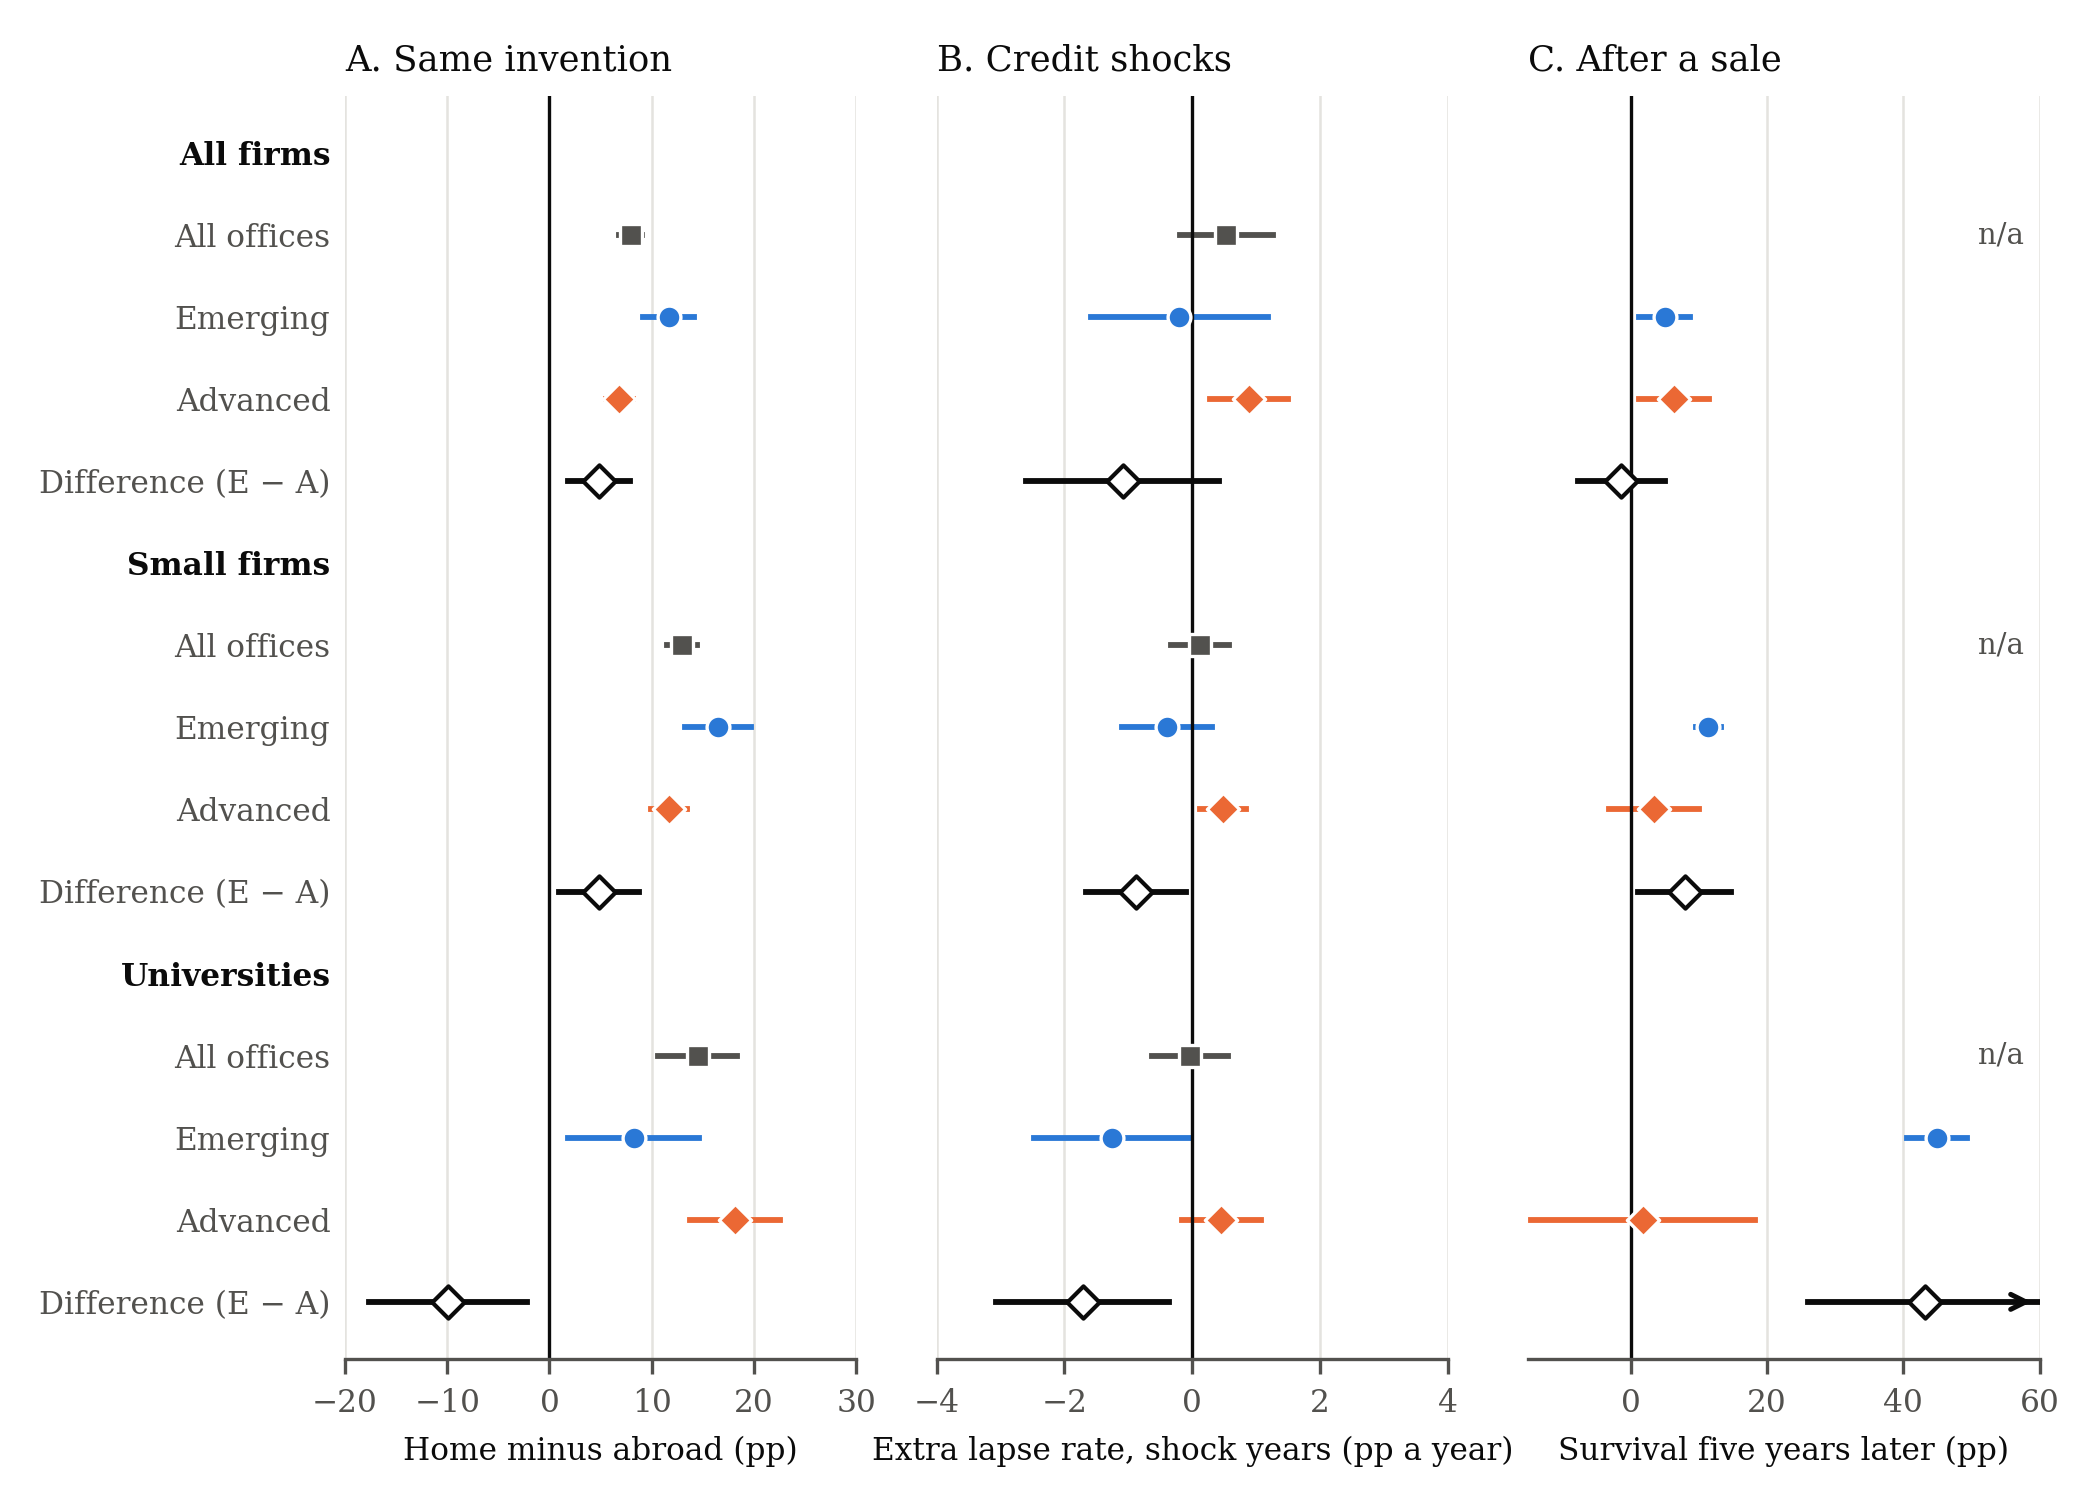
\includegraphics[width=\textwidth]{figures/fig5_constraints.png}
\caption{Three tests for owner constraints}\label{fig:constraints}
\figurenotes{Point estimates with 95\% confidence intervals, in percentage points. Squares: all offices; circles:
emerging economies; diamonds: advanced economies; open diamonds: emerging minus advanced. Small firms: 1--9 inventions
filed worldwide in 2000--2005 by the owner. A: survival eight years after grant of the home patent minus
that of the same invention's patents in other study offices; inventions granted at home and in at least one other
study office, with patent-family and office $\times$ year effects. B: extra yearly lapse rate of domestic owners in
credit-shock years; patents at risk by office, year, age and citation tercile, weighted by patents at risk, with
office $\times$ year, office $\times$ age $\times$ citation-tercile and office $\times$ owner-group $\times$ domestic
effects and standard errors clustered by office $\times$ year. Credit-shock years (systemic banking crises in
\citealp{LaevenValencia2018} and documented credit crunches): 2008--09 in the advanced economies, Taiwan and the
Czech Republic; 2003--04 (credit-card crisis; \citealp{KangMa2009}) and 2008--09 in Korea; 2013 (interbank crunch;
\citealp{BIS2013}) and 2017--18 (deleveraging) in China; 2008--09 and 2014--15 (rouble crisis) in Russia. C: survival
five years later of domestic owners' patents sold to an unrelated buyer 4--8 years after filing minus that of unsold
patents at the same point; emerging: China; advanced: Germany and France, the records that name the new
owner; patents alive and unsold 4--8 years after filing, with landmark-age $\times$ year, field and
owner-group effects, log citations up to the landmark and the grant lag. A and C: standard errors clustered by
owner. Emerging-minus-advanced differences are interactions in one regression.}
\end{figure}

\paragraph{Same invention, home and abroad.} Inventions patented both at home and in another study office hold the
technology fixed. With patent-family fixed effects, owners everywhere keep the home patent longer than the same
invention's foreign patents, by 7.9 points, and small firms by 13.0: the home market is where they use the invention,
and foreign protection is dropped first (panel A). If emerging-market owners found their home patents hard to use,
their home advantage would be smaller. It is larger: 11.7 points against 6.8 in the advanced economies, a difference
of 4.8, and 16.5 against 11.7 for small firms, a difference of 4.9.

\paragraph{Credit shocks.} If finance were binding, credit crunches should raise domestic owners' lapses, and small
firms' most. Following each patent year by year, with country-specific shock years (the notes to Figure~\ref{fig:constraints}), domestic
owners in the advanced economies lapse slightly more in shock years, by 0.9 points a year, and their small firms by 0.5
(panel B). Domestic owners in the emerging economies do not: $-0.2$ for all firms and $-0.4$ for small firms, so the
difference is negative ($-0.9$ for small firms). Each comparison is within an office and year, so fee changes and
recording practices do not drive it.

\paragraph{Sales.} One result points to owner capacity at the margin. I follow patents alive and not yet sold 4--8
years after filing, compare those sold in the next year with those not sold, and record whether they are alive five
years later. Many recorded transfers are renames, restructurings or moves within a group, which say nothing about a
new owner, so I keep only sales to unrelated buyers, identified from the owners' names; only the Chinese, German and
French records carry them (Supplemental Appendix Table~S5). A sale to an unrelated buyer raises the survival of small
Chinese firms' patents by 11.4 points, against 3.5 in Germany and France, a difference of 7.9.
Buyers pick good patents everywhere, so the premium itself does not measure what a sale adds; the informative part is
how much larger it is for small Chinese firm sellers. Because few small German and French firms sell to unrelated
buyers, the difference is imprecise; counted from grant it is 3.7, and with all recorded transfers in the six
offices that record them, 7.0. For mid-sized and large firms there is no difference.

\paragraph{Universities.} Universities behave differently from firms on two of the three tests. Emerging-market
universities keep the home patent 8.2 points longer than the same invention's foreign patents, against 18.2 for
advanced-economy universities, a difference of $-9.9$: unlike firms, they lean less on their home patents. And a sale
to an unrelated firm raises the survival of Chinese university patents by 44.9 points, against almost nothing in
Germany and France. Patents that Chinese universities would have dropped survive in the hands of firms; buyers choose
which patents to buy, so part of the gap is selection, but the same selection operates in the advanced economies,
where there is no premium. Credit shocks do not raise universities' lapses in either group as a whole, as expected for
owners funded by public budgets rather than credit. Together with their lower survival and values at equal quality,
this suggests that for Chinese universities the problem lies partly with the owner: they hold patents that firms find
worth keeping but that they do not use themselves.

\paragraph{Fees.} Fee changes test the cash constraints at renewal time directly, but only small firms receive the
discounts, so the test is small against large firms rather than emerging against advanced. China's fee reduction for
small owners (70\% in the first three fee-years after grant, raised to 85\% and extended to six fee-years in 2016 and
to ten in 2018) barely changes small firms' lapses: a 10\% lower fee lowers their lapse rate, 3.6\% a year, by about
0.2\% of its level, not significantly, measured over all eligible firms because take-up is not observed. Small US
firms respond to changes in the three US maintenance fees about ten times as strongly (2.6\% for a 10\% fee change). Small Chinese firms are not
more fee-sensitive than small US firms.
